\subsection{An illustrate of deconvolution}

Here the prolongation operator is also corresponded to some
well-know operators in CNN which is often called as: deconvolution, transposed convolution or even up-pooling.


\subsubsection{Recall convolution in 1D}
Suppose the input data is denoted as $X$, the kernel for the convolution layer is $K_1$. We can obtain the encoded output $Y$ by convolution as
\begin{align}
    K_1 \ast X  = Y.
\end{align}

If we rewrite the convolution in the form of matrix multiplication, it becomes
\begin{align}
   Y = K_1 \ast X = T \cdot X.
\end{align}
For the purpose of illustration, we take $K_1 \in \mathbb{R}^4$, $X \in \mathbb{R}^8$ with the stride  2 without padding. Then we have $Y \in \mathbb{R}^5$ and $T \in \mathbb{R}^{5*8}$.

Suppose $K_1=(k_1, k_2, k_3, k_4)$ and $X=(x_1, x_2, ..., x_8)$. The corresponding coefficient matrix $T$ can be represented as 
\begin{align}
   T = \mathcal S \cdot \tilde{T} &= 
%  \begin{bmatrix}
%    (1-2r)  & -r      & 0       & \cdots  & 0  \\
%    -r      & (1-2r)  & -r      & \ddots  & \vdots   \\
%     0      &  \ddots & \ddots  & \ddots  & 0  \\
%    \vdots  &         & -r      & (1-2r)  & -r  \\
%     0      & \cdots  & 0       & -r      & (1-2r)
%  \end{bmatrix}
\left(
  \begin{array}{ccccccccc}
     1 & 0 & 0 & 0 & 0 & 0 & 0 & 0 & 0 \\
     0 & 0 & 1 & 0 & 0 & 0 & 0 & 0 & 0 \\
     0 & 0 & 0 & 0 & 1 & 0 & 0 & 0 & 0 \\
     0 & 0 & 0 & 0 & 0 & 0 & 1 & 0 & 0 \\
     0 & 0 & 0 & 0 & 0 & 0 & 0 & 0 & 1 \\
  \end{array}
\right)_{5*9}
\left(
  \begin{array}{cccccccc}
     k_3 & k_4 & 0 & 0 & 0 & 0 & 0 & 0  \\
     k_2 & k_3 & k_4 & 0 & 0 & 0 & 0 &  0 \\
     k_1 & k_2 & k_3 & k_4 & 0 & 0 & 0 & 0  \\
     0 & k_1 & k_2 & k_3 & k_4 & 0 & 0 & 0  \\
     0 & 0 & k_1 & k_2 & k_3 & k_4 & 0 & 0  \\
     0 & 0 & 0 & k_1 & k_2 & k_3 & k_4 & 0  \\
     0 & 0 & 0 & 0 & k_1 & k_2 & k_3 & k_4  \\
     0 & 0 & 0 & 0 & 0 & k_1 & k_2 & k_3   \\
     0 & 0 & 0 & 0 & 0 & 0 & k_1 & k_2  \\
  \end{array}
\right)_{9*8}\\ \notag 
&= 
\left(
  \begin{array}{cccccccc}
     k_3 & k_4 & 0 & 0 & 0 & 0 & 0 & 0  \\
     k_1 & k_2 & k_3 & k_4 & 0 & 0 & 0 &  0 \\
     0 & 0 & k_1 & k_2 & k_3 & k_4 & 0 &  0  \\
     0 & 0 & 0 &0 & k_1 & k_2 & k_3 & k_4   \\
     0 & 0 & 0 & 0 & 0 & 0 & k_1 & k_2    \\
  \end{array}
\right)_{5*8}.
\end{align}
Here $\mathcal S$ denote the operation of stride being 2 and $\tilde{T}$ is the standard convolution operation.

The procedure can be illustrated as below.
\begin{figure}[htbp]
\centering{
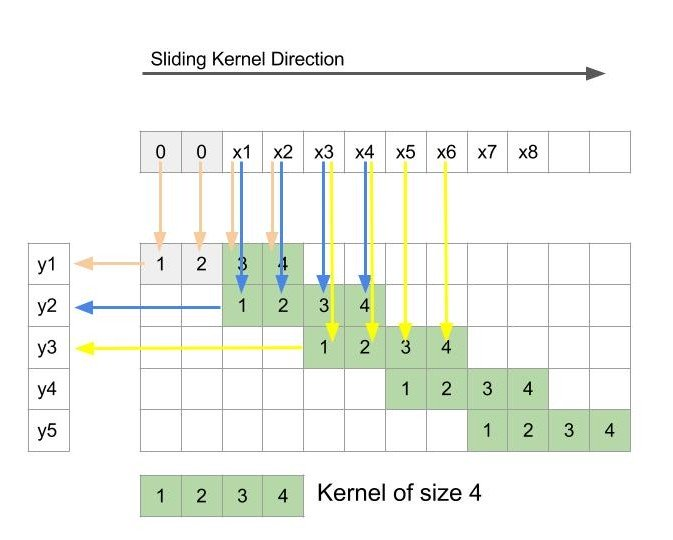
\includegraphics[width=.6\textwidth]{conv.jpeg}}
\caption{Depiction of usual convolution process with 1-d input}
\end{figure}


\subsubsection{Deconvolution in 1D as example}
Suppose the data is denoted as $Y$ and the wanted output as $\tilde{X}$. 
In TensorFlow, $\tilde{X}$ is obtained from $Y$ with the function tf.nn.conv3d$\_$transpose. 
Similar case can be found in PyTorch as: torch.nn.ConvTranspose2d.

For example, here is what tf.nn.conv3d$\_$transpose does.
It construct another CNN with a convolution layer only, which takes $Y$ as 
the output and $\tilde{X}$ as the input. Then  the input is updated with the 
backpropagation by the function gen$\_$nn$\_$ops.conv3d$\_$backprop$\_$input$\_$v2. 
%This function does the following operation.

If we rewrite the deconvolution in the form of matrix multiplication, it becomes
\begin{align}
   \tilde{X} = K_2 \ast Y = T^\top \cdot Y.
\end{align}

%Suppose $Y$ can be obtained by convolution as
%\begin{align}
%    K_2 \ast \tilde{X}  = Y.
%\end{align}
%Then with the backpropagation, the input and the parameters can be updated as
%\begin{align}
%   dY \ast(K_2)^\top  = d\tilde{X},   \\
%   dY \ast \tilde{X}      = dK_2.
%\end{align}
%After $\tilde{X}$ is updated, the $L^2$ loss function is used to compute the difference between $X$ and $\tilde{X}$. 

With the same notation as above, the corresponding coefficient matrix $T^\top$ can be represented as 
\begin{align}
   T^\top = \tilde{T}^\top\cdot  \mathcal S^\top &= 
%  \begin{bmatrix}
%    (1-2r)  & -r      & 0       & \cdots  & 0  \\
%    -r      & (1-2r)  & -r      & \ddots  & \vdots   \\
%     0      &  \ddots & \ddots  & \ddots  & 0  \\
%    \vdots  &         & -r      & (1-2r)  & -r  \\
%     0      & \cdots  & 0       & -r      & (1-2r)
%  \end{bmatrix}
\left(
  \begin{array}{ccccccccc}
     k_3 & k_2 & k_1 & 0 & 0 & 0 & 0 & 0  & 0\\
     k_4 & k_3 & k_2 & k_1 & 0 & 0 & 0 &  0 & 0\\
     0 & k_4 & k_3 & k_2 & k_1 & 0 & 0 & 0 & 0\\
     0 & 0 & k_4 & k_3 & k_2 & k_1 & 0 & 0  & 0\\
     0 & 0 & 0 & k_4 & k_3 & k_2 & k_1 & 0  & 0\\
     0 & 0 & 0 & 0 & k_4 & k_3 & k_2 & k_1  & 0\\
     0 & 0 & 0 & 0 & 0 & k_4 & k_3 & k_2 & k_1  \\
     0 & 0 & 0 & 0 & 0 & 0  & k_4 & k_3 & k_2   \\
  \end{array}
\right)_{8*9}
\left(
  \begin{array}{ccccc}
     1 & 0 & 0 & 0 & 0  \\
     0 & 0 & 0 & 0 & 0  \\
     0 & 1 & 0 & 0 & 0  \\
     0 & 0 & 0 & 0 & 0  \\
     0 & 0 & 1 & 0 & 0  \\
     0 & 0 & 0 & 0 & 0  \\
     0 & 0 & 0 & 1 & 0  \\
     0 & 0 & 0 & 0 & 0  \\
     0 & 0 & 0 & 0 & 1  \\
  \end{array}
\right)_{9*5}
\\ \notag 
&= 
\left(
  \begin{array}{ccccc}
     k_3 & k_1 & 0 & 0 & 0   \\
     k_4 & k_2 & 0 & 0 & 0   \\
     0 & k_3 & k_1 & 0 & 0  \\     
     0 & k_4 & k_2 & 0 & 0  \\
     0 & 0 & k_3 & k_1 & 0  \\
     0 & 0 & k_4 & k_2 & 0  \\
     0 & 0 & 0 & k_3 & k_1  \\
     0 & 0 & 0 & k_4 & k_2  \\
  \end{array}
\right)_{8*5}.
\end{align}
Here $\mathcal S^\top$ denote the operation of padding(adding zeros) and $\tilde{T}$ is the standard deconvolution operation.

The procedure can be illustrated as below.
\begin{figure}[htbp]
\centering{
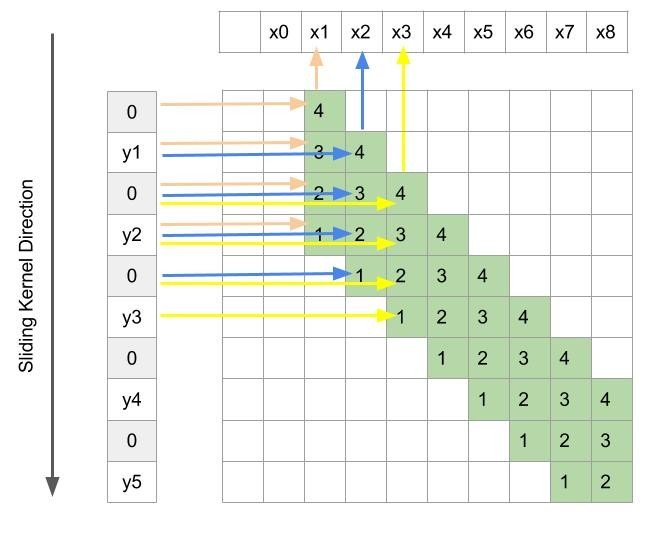
\includegraphics[width=.6\textwidth]{deconv.jpeg}}
\caption{Deconvolution}
\end{figure}

\subsection{Some linear and nonlinear mappings and extractors}
A data-feature map $A$ and feacture extractor $B$ can be either
linear or nonlinear.   The nonlinearity can be obtained from
appropriate application of an activation function
\begin{equation}
\label{act}
\sigma: \mathbb{R} \to \mathbb{R} .
\end{equation}
In this paper, we mainly consider a special activation function, known 
as the {\it rectified linear unit} (ReLU), which is defined by
\begin{equation}
\label{relu}
\sigma(x)= {\rm ReLU}(x) :=\max(0,x), \quad x\in\mathbb{R}. 
\end{equation}
By applying the function to each component, we can extend this
\begin{equation}
\label{vector-act}
\sigma:\mathbb R^{m\times n\times c}\mapsto \mathbb R^{m\times n\times c}.  
\end{equation}


A linear data-feature mapping can simply given by a convolution as in \eqref{con1}:
\begin{equation}
\label{linearA}
A(f)=\xi\ast f
\end{equation}
A nonlinear mapping can be given by compositions of convolution and
activation functions:
\begin{equation}
\label{nonlinearA}
A=\xi\circ\sigma\circ\eta ,
\end{equation}

and 
\begin{equation}
\label{extractor}
B=\sigma\circ \gamma \circ\sigma  .
\end{equation}
Here $\xi$, $\eta$ and $\gamma$ are all 
appropriate convolution mappings.


\subsection{An iterative feacture extraction scheme}
One key idea in this paper is that we use a simple iterative
process to approximately solve \eqref{Auf} using \eqref{vBf}. Namely,
for $i=1:\nu$
\begin{equation}\label{eq:smoothB}
u^{i} = u^{i-1} + B^{i}(f- A(u^{i-1})) 
\end{equation}
for an appropriately chosen $u^0$.  We refer to \cite{xu1992iterative}
for more discussion on iterative scheme in the form of \eqref{eq:smoothB}.


